%=================================================================
% This template is based on IMRT Latex template by Eric A. Mueller
%================================================================= 

\documentclass[10pt,twoside,a4paper]{report}

 \usepackage[bt,fs,english]{ethasl}   % New styles and commands
                                      % Options: 	bt/mt: Bachelorthesis/Masterthesis
                                      %						fs/hs: Fr�hlingssemester/Herbstsemester
                                      %						german/english: Deutsch/English

% \includeonly{}                      % Quick formatting
% \usepackage[draft]{graphicx}        % Quick formatting

 \usepackage{a4}                      % Paper size
 \usepackage[latin1]{inputenc}        % Keybord settings
 \usepackage{amsmath}                 % Additional math functionality
 \usepackage{amssymb}                 % Additional math functionality
 \usepackage{graphicx}                % EPS figures
 \usepackage[dvips]{epsfig}           % EPS figures
 \usepackage{float}                   % Placement of floating objects
 \usepackage{fancyhdr}                % Headings
 \usepackage{rotating}
 \usepackage{multirow}
 \usepackage{url}
 \usepackage{colortbl}
 \usepackage{ifpdf}
 

 \usepackage{hyperref}
 \usepackage{color}
 \definecolor{black}{rgb}{0,0,0}
 \definecolor{white}{rgb}{1,1,1}

 \definecolor{darkred}{rgb}{0.5,0,0}
 \definecolor{darkgreen}{rgb}{0,0.5,0}
 \definecolor{darkblue}{rgb}{0,0,0.5}

 \hypersetup{colorlinks
	,linkcolor=black
	,filecolor=black
	,urlcolor=black
	,citecolor=black
 }


 \ifpdf
	\usepackage[update]{epstopdf}
 \else
 \fi

 \usepackage{german}                  % German language "o, "a, use.
%\usepackage{ae}                      % German specials

%---------------------------------------------------------------------------

 \setlength{\parindent}{0em}                   % Disable parindent
 \rhead[\thepage]{\nouppercase{\rightmark}}    % Special headings
 \lhead[\nouppercase{\leftmark}]{\thepage}     % Special headings
 \cfoot{}                                      % Special headings

%---------------------------------------------------------------------------

 \title{Human-Machine Interface for Operating a Blimb}
 %\subtitle{bla bla bla}

 
 \studentA{Krebs Matthias}
 \studentB{Ledergerber Anton}
% \studentC{Student 3}
 
 

\supervisionA{Konrad Rudin}
\supervisionB{Mora Javier Alonso}
\supervisionC{Paul Beardsley XXXXX}
 

%===========================================================================
\begin{document}

%---------------------------------------------------------------------------
% Title page

 \maketitle
 \pagestyle{plain}
 \pagenumbering{roman}

%---------------------------------------------------------------------------
% Declaration of Originality

\pagestyle{empty}
% TODO Modify placeholders in declaration.tex
\include{declaration}

%---------------------------------------------------------------------------
% Preamble

 %!TEX root = Bericht.tex
%---------------------------------------------------------------------------
% Preface

%\chapter*{Vorwort}

%Bla bla \dots

 %\cleardoublepage

%---------------------------------------------------------------------------
% Table of contents

 \setcounter{tocdepth}{2}
 \tableofcontents

 \cleardoublepage

%---------------------------------------------------------------------------
% Abstract

%\chapter*{Zusammenfassung}
% \addcontentsline{toc}{chapter}{Zusammenfassung}

%Bla bla \dots

% \cleardoublepage

\chapter*{Abstract}
 \addcontentsline{toc}{chapter}{Abstract}

Hier kommt der Abstact hin \dots

 \cleardoublepage

%---------------------------------------------------------------------------
% Acknowledgements

%\chapter*{Acknowledgements}\label{chap:Acknowledgements}
% \addcontentsline{toc}{chapter}{Acknowledgements}
\chapter*{Acknowledgements}
 \addcontentsline{toc}{chapter}{Acknowledgements}

Without the help of a few people this thesis would not have been possible. We received the necessary support from all sides throughout the project to realize the this HMI which we are proud of.

Prof. Dr. Roland Y. Siegwart\\
Dr. Paul Beardsley\\
PhD students Konrad Rudin and Javier Alonso Mora\\
Gerhard R"othlin\\
Lorenz Meier\\
Alexander Rudyk\\



 \cleardoublepage

%---------------------------------------------------------------------------
% Symbols

%\chapter*{Symbolverzeichnis}\label{chap:symbole}
% \addcontentsline{toc}{chapter}{Symbolverzeichnis}
\chapter*{Symbols}\label{chap:symbole}
 \addcontentsline{toc}{chapter}{Symbols}

%\section*{Symbole}
\section*{Symbols}
\begin{tabbing}
 \hspace*{3cm} \= \kill
  $\phi, \theta, \psi$ 					\> roll, pitch and yaw angle \\[0.5ex] 					
  $b$								\> gyroscope bias \\[0.5ex]						
  $\Omega_m$						\> 3-axis gyroscope measurement \\[0.5ex]
  $G^h$   							\> geometrical continuity of a curve \\[0.5ex]
  $C^h$							\> parametric continuity of a curve \\[0.5ex]
 \end{tabbing}

%\section*{Indizes}
\section*{Indices}
\begin{tabbing}
 \hspace*{1.6cm}  \= \kill
 $x$ \> x axis \\[0.5ex]
 $y$ \> y axis \\[0.5ex]
 
\end{tabbing}

%\section*{Akronyme und Abk�rzungen}
\section*{Acronyms and Abbreviations}
\begin{tabbing}
 \hspace*{1.6cm}  \= \kill
 ETH \> Eidgen�ssische Technische Hochschule \\[0.5ex]
 EKF \> Extended Kalman Filter \\[0.5ex]
 IMU \> Inertial Measurement Unit \\[0.5ex]
 UAV \> Unmanned Aerial Vehicle \\[0.5ex]
 UKF \> Unscented Kalman Filter \\[0.5ex]
\end{tabbing}

 \cleardoublepage

%---------------------------------------------------------------------------


 \pagestyle{headings}                 % Default headings
 \pagestyle{fancy}                   % Special headings
 \pagenumbering{arabic}

%---------------------------------------------------------------------------
% Chapters

 \chapter{Introduction}\label{sec:introduction}

%\section{Motivation}

\section{Context}

\section{Goals}

\section{System Overview}

\section{Similar Systems and their HMI}

\section{Structure of the Report}
 \cleardoublepage
 \include{chapter}
 \cleardoublepage
 
\chapter{Finding a Hardware and Software Solution}
References to \cite{kammermann}
\subsection{Requirements}
\subsection{Existing Solutions}
\subsection{Realization}
 \cleardoublepage
 %!TEX root = Bericht.tex
\graphicspath{{graphics/HMI/}{graphics/control_modes/}}
\chapter{The different Control Modes}
\label{cha:DifferentControlModes}

\begin{table}[H]		% [H] indicates that the table should be right here.
	\begin{tabular}{c c c c c} %{p{0.16\textwidth}p{0.16\textwidth}p{0.16\textwidth}p{0.16\textwidth}p{0.16\textwidth}}	% add p{size_of_column} for every new column you'd like to have. If you put a | between the p then there is a vertical line between the columns. 
	Test Phase 		& Direct Control 	& Assisted Control 	& Half Automatic	& Full Automatic  \\
	\toprule[1.25pt]				%define the line thickness of the top rule
	Thrust 1		& Thrust $x$	& Velocity $x$	& Velocity	& Velocity	\\
	Thrust 2		& Thrust $y$	& \textit{Velocity $y$}	& Rotation $x$	& Rotation $x$\\
	Thrust 3		& Thrust $z$	& \textit{Velocity $z$}	& Rotation $y$	& Waypoints	\\
	Thrust 4		& Moment $x$	& Rotation $x$	& Rotation $z$	&	Camera target\\
	Direction 1		& Moment $y$	& Rotation $y$	& Waypoints	&	\\
	Direction 2		& Moment $z$	& Rotation $z$	&		&	\\
	Direction 3		& 		& 		&		&	\\
	Direction 4		& 		& 		&		&	\\

	\bottomrule[1.25pt]
	\end{tabular} 
	\caption[The different control modes]{With the control modes, different inputs are given to the controller. The inputs in \textit{italic} are not available for \textit{Assisted RC  Control}.}
	\label{table:control_modes}
\end{table}

\begin{figure}[H] % [H] steht dafür, dass das Bild genau hier im Text sein soll.
	\begin{center}
		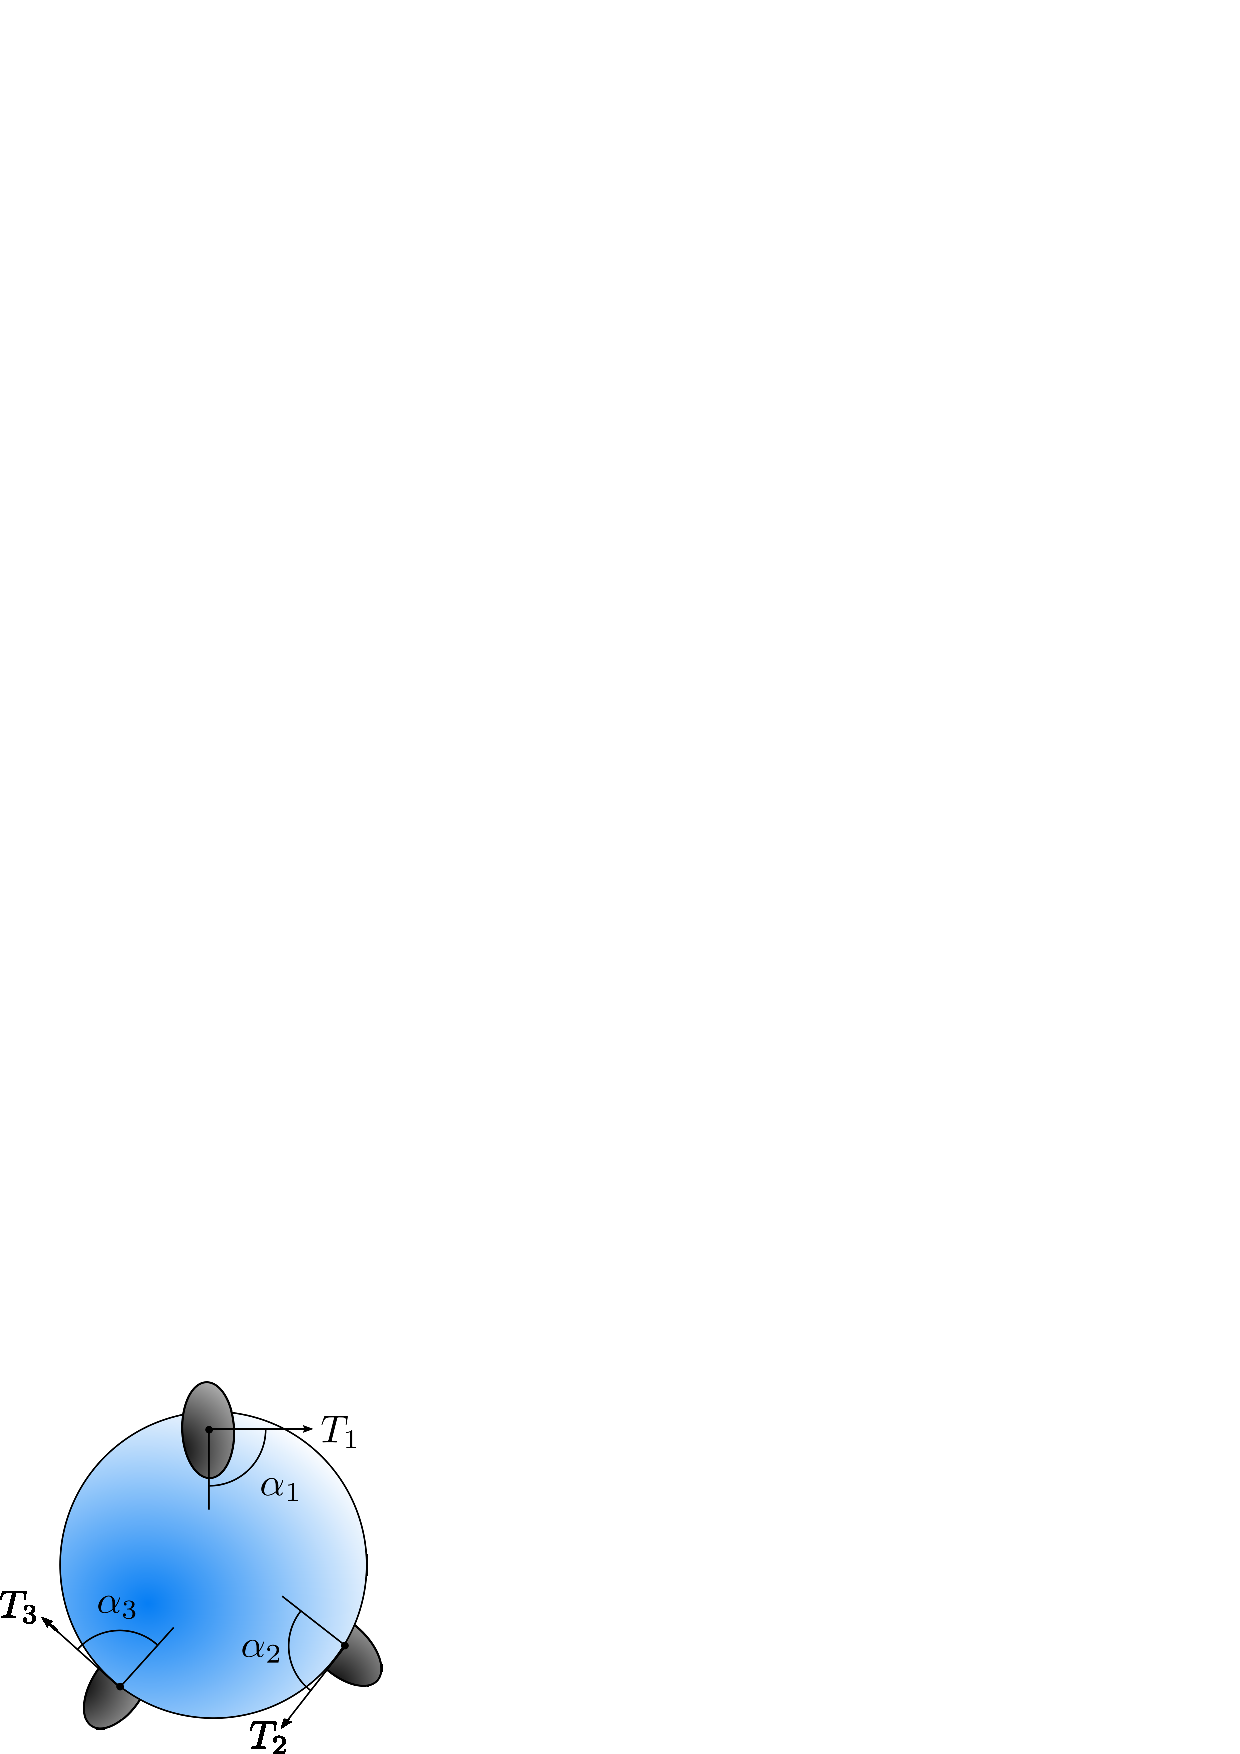
\includegraphics[width=0.3\textwidth]{TPC.pdf}
		\caption[Test Phase]{Test Phase}  
		\label{figure:test_phase}		
	\end{center}
\end{figure}

\begin{figure}[H] % [H] steht dafür, dass das Bild genau hier im Text sein soll.
	\begin{center}
		\includegraphics[width=0.3\textwidth]{DC.pdf}
		\caption[Direct control]{Direct Control}  
		\label{figure:direct_control}
	\end{center}
\end{figure}

\begin{figure}[H]		
	\small{
		\begin{center}
			\parbox{0.25\textwidth}{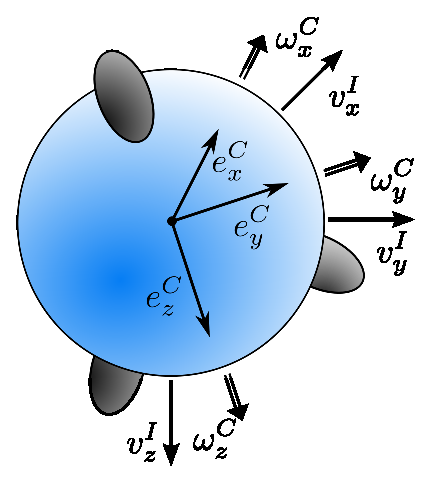
\includegraphics[width=0.25\textwidth]{AC}
			 Assisted Control}
			\hspace{0.1\textwidth}			
			\parbox{0.25\textwidth}{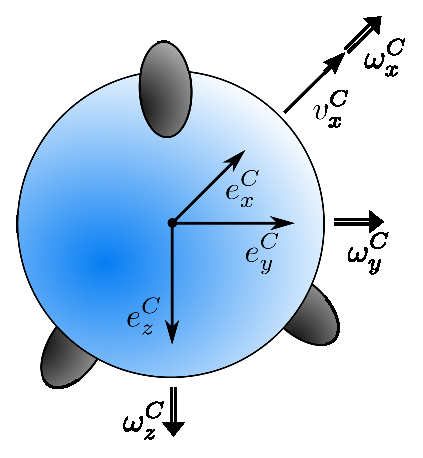
\includegraphics[width=0.25\textwidth]{RC}
			Assisted RC Control}
	\caption[Assisted Control]{Assisted Control with controlling six (left) and four (right) stabilized degrees of freedom.}
		\label{figure:assisted_control}
		\end{center}
	}			
	\vspace{4.5mm}
\end{figure}

\begin{figure}[H] % [H] steht dafür, dass das Bild genau hier im Text sein soll.
	\begin{center}
		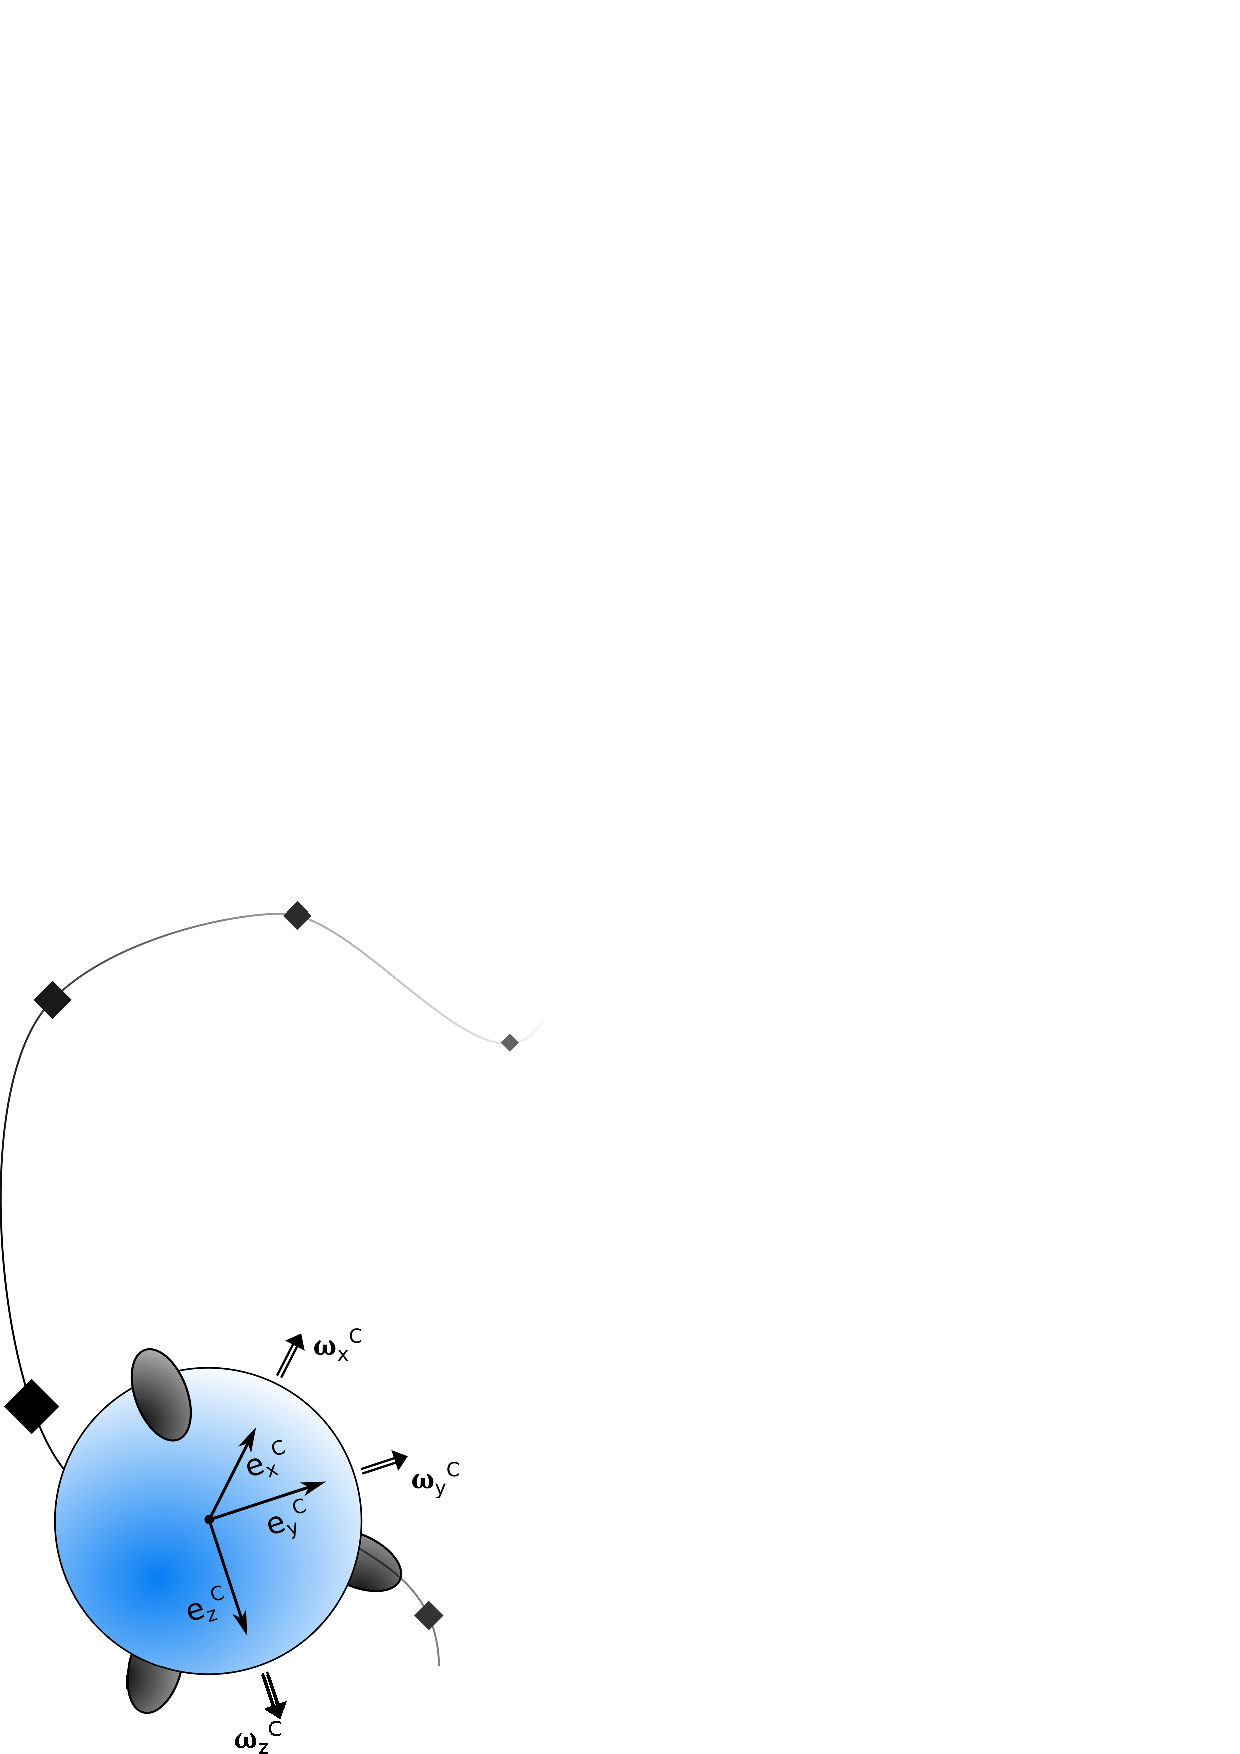
\includegraphics[width=0.4\textwidth]{HAC.pdf}
		\caption[Half automatic control]{Half Automatic Control}  
		\label{figure:half_automatic_control}		
	\end{center}
\end{figure}


\begin{figure}[H] % [H] steht dafür, dass das Bild genau hier im Text sein soll.
	\begin{center}
		\includegraphics[width=0.4\textwidth]{FAC.pdf}
		\caption[Full automatic control]{Full Automatic Control.}  
		\label{figure:full_automatic_control}		
	\end{center}
\end{figure}


\section{Elaboration}
\label{sec:elaboration}
\textit{About the need of different modes, the requirements of image capturing and overview of the realized modes}
\section{Manual Control Modes}
\label{manualControlModes}
\textit{Direct Control and Assisted Control}
\section{Automatic Control Modes}
\label{automaticControlModes}
\textit{Half Automatic Control and Full Automatic Control}
 \cleardoublepage
 
\chapter{Realization of the HMI as a whole and for each Control Mode}
 \cleardoublepage
 \chapter{Trajectory Planning}
\label{cha:trajectory}
For the two most advanced modes, i. e. the Half-Automatic and the Full-Automatic Mode, trajectories had to be generated. In this chapter the best trajectories for \textsc{Skye} are elaborated.

%\subsection{Our Approach}
%From the GUI it was given that the goal trajectory would be a multipoint-interpolating %trajectory. The user is able to define waypoints on a map which afterwards should be %connected with a reasonable and realizable trajectory. Beside interpolating trajectories %there exist also approximating trajectories but they were not taken into consideration, since %usually the user wants skye fly directly through a waypoint.

%In another Bsc Thesis elaborated in this project a controller for waypoint following was %designed. So it was convenient in the scope of this Thesis to use this controller instead of %a specialized trajectory controller.

\section{Experimental Design}

\section{Definition of Trajectories}
\label{sec:definition}
\subsection{Paths and Trajectories}



\subsection{Interpolation and Approximation}
If one wants to draw a line through a set of data points, there exists two ways to do this. On the one hand the line must pass all data points no matter how many bends it will have, on the other hand the line tries to best fit the data, i.e. a function of a  certain order is adopted to best fit the date. E.g. this can be done with least-squares. If the pilot  defines the trajectory with a set of waypoints, i.e. data points, he usually wants the (UAV already defined?!!!!) to pass through all of them. Therefore the waypoints must be interpolated and not approximated with a suitable curve.

\textbf{(!!!Bsp Plot von interpolierenden und approximierenden funktionen!!!)}


\section{Spline Theory}
A set of data points can be interpolated with one single curve or with a set of curves defined over a certain interval.  For a 
\label{sec:splineTheory}
references to \cite{engeln}, \cite{biagiotti} and \cite{doessegger}
\subsubsection{Continuity}
\subsubsection{Boundary Conditions}
\subsubsection{Polynomial Order}
\subsubsection{Parametrization}
\subsection{Piecewise Polynomial Interpolating Splines}
\subsubsection{Boundary Conditions}
\subsubsection{Polynomial Order}
\subsubsection{Parameterization}
\subsection{B-Splines}
\subsubsection{Boundary Conditions}
\subsubsection{Polynomial Order}
\subsubsection{Parametrization}

\section{Trajectory Generation}
\label{sec:trajectoryGeneration}
\subsection{System Constraints}
\subsubsection{Maximum Velocities and Accelerations}
In order to plan a feasible trajectory one has to know the capabilities of the system. Here just a basic derivation for the velocities and accelerations is given, for more details refer to (!!!!Bsc Thesis Joe, Bsc Thesis Andy)\\

The maximum feasible acceleration in any direction is calculated to be:

\begin{equation}
  \left|a_{max} \right| =  \frac{\left|F_{res, w}\right|}{m_{tot}} = 0.96 m/s^2
\end{equation}

Whereas the $F_{res,w}$ is the force resulting from all four thrusters operated under full load in the worst direction and $m_{tot}$ is the sum of the masses of the helium, the virtual mass and the mass of the system itself.\\


The maximum feasible velocity in any direction is calculated to be:

\begin{equation}
\left|v_{max} \right| = \sqrt{\frac{\left|F_{res,w} \right|}{\frac{1}{2}c_d \rho \pi r^2}}=4.7 m/s
\end{equation}

which is nothing but $ \left|F_{res,min} \right| = \left|F_{dray} \right| $.\\

For trajectories for position and orientation the maximal feasible angular acceleration is also important. It is calculated to be:

\begin{equation}
  \left|\Psi_{max} \right| =  \frac{\left|M_{res,w}\right|}{\left| \lambda_{max, J_{B}} \right|} = 2.82 rad/s^2 
\end{equation}

which is quite conservative because it is assumed that worst axis for turning is also the principle axis of the inertia tensor with the highest inertia.\\

Since the system is almost undamped for rotations, the rotational velocities will never be the limiting factor.

\subsection{Time Parametrization}

\section{Controller Implementation}
\label{sec:controllerImplementation}
\subsection{Trajectory Controller}
see \cite{snider} and \cite{deluca}
\subsection{Pure Pursuit Position Controller}
see also \cite{snider}
\subsection{Cross Track Error Controller}
see \cite{williams}

\section{Discussion}
\label{sec:discussion}


 \cleardoublepage
% ...
%
%---------------------------------------------------------------------------
% Appendix

 \appendix
 %!TEX root = Bericht.tex
\chapter{Appendix}\label{cha:appendix}

\section{Parameterizations}
\subsection{Arc Length Distribution}
\label{subsec:arcLengthDistribution}
TO DO
\subsection{Effect of different Parameterizations with cubic, quartic and quintic splines}
\label{subsec:parameterization_degree}

\begin{figure}[H]
  \begin{minipage}[t]{0.9\textwidth}
    \includegraphics[width = \textwidth]{graphics/Parameterization345_road_agile.eps}
  \end{minipage}
  \caption{The different parameterizations shown with cubic, quartic and quintic splines}
  \label{fig:parameterization_cqq}
\end{figure}

 %\cleardoublepage


%\chapter{Nochmals irgendwas}\label{sec:nochirgendwas}

%Bla bla \dots

 %\cleardoublepage

%
%---------------------------------------------------------------------------
% Literature

 %!TEX root = Bericht.tex
\begin{thebibliography}{99}
%\addcontentsline{toc}{chapter}{Literaturverzeichnis}
\addcontentsline{toc}{chapter}{Bibliography}



%\bibitem {comfilt} {\sc R.~Mahony, T.~Hamel, J.-M.~Pflimlin}:
%{\it Complementary filter design on the special orthogonal group SO(3)}. In 45th Conference
%on Decision and Control CDC'05, Seville, Spain, 2005.
\bibitem{schaffnervu}{\sc A.~Schaffner, N.~Vuilliomenet}:
{\it Blimp Actuation Chain Modeling and Optimization}. BSc thesis, ETH Zurich, 2012.
\bibitem {weichart} {\sc J.~Weichart}:
{\it Agile Blimp Modeling and Simulation Environment}. BSc thesis, ETH Zurich, 2012.
\bibitem {kammermann} {\sc T.~Kammermann}:
{\it Evaluation and implementation of a control device for a ballbot}. BSc thesis, ETH Zurich, 2010.
\bibitem {meiermueri} {\sc D.~Meier, L.~M{\"u}ri}:
{\it Agile Blimp Controller Design}. BSc thesis, ETH Zurich, 2012.
\bibitem{burri}{\sc M.~Burri}:
{\it Communication Software for a Blimp}. BSc thesis, ETH Zurich, 2012.
\bibitem{blanchette}{\sc J.~Blanchette, M~Summerfield}:
{\it C++ GUI Programming with Qt 4}. Prentice Hall, Upper Saddle River, N.J., 2010.
\bibitem {snider} {\sc J. M.~Snider}:
{\it Automatic Steering Methods for Autonomous Automobile Path Tracking}. Research Report CMU-RI-TR-09-08, Robotics Institute Carnegie Mellon University Pittsburgh, Pennsylvania, 2009.
\bibitem{dahmen}{\sc W.~Dahmen, A.~Reusken}:
{\it Numerik f{\"u}r Ingenieure und Naturwissenschaftler}. Springer Verlag, Berlin, 2006.
\bibitem{stammbach}{\sc U.~Stammbach}:
{\it Analysis I/II, Teil A}. ETH Zurich, 2005.
\bibitem{haron}{\sc H. Haron, [et al.]}:
{\it Parameterization Method on B-Spline Curve}. Mathematical Problems in Engineering, vol. 2012.
\bibitem{lee}{\sc E.T.Y.~Lee}:
{\it Choosing nodes in parametric curve interpolation, Computer-Aided Design}. pages 363-370, (http://www.sciencedirect.com/science/article\-/pii/0010448589900031), 1989.
\bibitem {doessegger} {\sc S.~D{\"o}ssegger}:
{\it Time-optimal trajectories for a Ballbot}. BSc thesis, ETH Zurich, 2010.
\bibitem{mellinger}{\sc D.~Mellinger, V.~Kumar}:
{\it Minimum Snap Trajectory Generation and Control for Quadrotors}.IEEE International Conference on robotics and Automation, Shanghai, 2011.
\bibitem {biagiotti} {\sc L.~Biagiotti, C.~Melchiorri}:
{\it Trajectory Planning for Automatic Machines and Robots}. Springer Verlag, 2008.
\bibitem {engeln} {\sc G.~Engeln-M{\"u}llges, K.~Niederdrenk, R.~Wodicka}:
{\it Numerik-Algorithmen : Verfahren, Beispiele, Anwendungen}. Springer Verlag, 2011.
\bibitem {williams} {\sc D. L.~Williams}:
{\it Loitering Behaviors of Autonomous Underwater Vehicles}. MSc thesis, Naval Postgraduate School, Monterey, California, 2002.
\bibitem {deluca} {\sc A.~De Luca, G.~Oriolo, C.~Samson}:
{\it Feedback Control of a Nonholonomic Car-Like Robot}. In Robot Motion Planning and Control, pages 171-249, 1998.


%\bibitem{won}{\sc Won Y.~Yang,  [et al.]}:
%{\it Applied Numerical Methods Using MATLAB} . Wiley-Interscience, Hoboken, 2005.

\end{thebibliography}


%---------------------------------------------------------------------------

\end{document}
%===========================================================================
